\documentclass[12pt, a4paper]{report}
\usepackage[T1]{fontenc}
\usepackage{inputenc}
\usepackage{pdfpages}
\usepackage[toc]{glossaries}

\makeglossaries
\newglossaryentry{computer}
{
  name=computer,
  description={is a programmable machine that receives input,
               stores and manipulates data, and provides
               output in a useful format}
}

\usepackage{tabularx}
	\newcolumntype{L}{>{\raggedright\arraybackslash}X}


\begin{document}
\title{}
\author{Linda Boedi and Valentin Bossi\\
ZHAW School of Engineering}
\date{}

\maketitle
\tableofcontents

\chapter{Summary}

\chapter{Introduction}

\chapter {Competitor Analysis}
\section{Optical versus acoustical measurement}
To measure the frequency of the balance wheel of a mechanic clock there exist mainly two methods on the market, acoustical and optical measurement. The common used method is by analyzing the noises of the balance wheel. More expensive devices use both acoustical and optical feedback.

\begin{table}
 \centering
\begin{tabularx}{\linewidth}{ |c||L|L|  }
 \hline
 \multicolumn{3}{|c|}{\textbf{Comparison acoustical and optical measurement}} \\
 \hline
 & \textbf{acoustical}  & \textbf{optical} \\\hline
  since   &  around 19th century (2)  & end of 20th century (2)\\ \hline
 accuracy &   0.1 s/d & 0.1 s/d\\  \hline
 advantages & most experience (exists for about 200 years)& measurement can be done anywhere\\  \hline
 disadvantages & background noises need to be filtered out& \\
 \hline
\end{tabularx}
    \end{table}

\subsection{Acoustical measurement}
The first used method to get the frequency measurement of the balance wheel was by using a vibrograph was used. For every "tick" of the clock a line was drawn onto a ongoing strip of paper. Out of the distance between of these lines the frequency was calculated. (1) But as this method isn't the most accurate other techniques are used nowadays.  
Modern watch timing machines use an oscillating quartz crystal as comparison for the frequency of the balance wheel (1). The noises of the balance wheel are recorded and amplified with a microphone whereat unwanted background noises need to be filtered out. 

\subsection{Optical measurement}
About hundred years later, optical watch timing machines joined the acoustical ones. There are barely devices on the market, which use only optical measurement, but several companies started to combine their acoustical with optical metering. One way to scale the frequency of the balance wheel optically is by using a laser. The beam will be periodically interrupted by the balance wheel and thus the frequency can be calculated (3). In this paper we want to try to quantify the frequency optically by using image processing. There is hardly to none company out there, which uses the last technique for measuring the frequency.

\subsection{Companies}
\subsubsection{Witschi - WisioScope S}
WisioScope S tests mechanical watches acoustically and optically. The measurement is done parallel and in this way is more accurate as both signals are used for the calculation of the frequency.
The optical metering is done using a laser and lighting, a camera helps to adjust the watch properly. The costs of their product are: CHF 10450.-

\subsubsection{Lepsi - WatchScope/WatchAnalyzer}
The WatchScope and WatchAnalyzer by Lepsi are mostly for enthusiasts and not really for the manufacturing. Both devices only work with acoustical input. All data can be accessed with the smartphone. The prices of their product are CHF 369.-, resp. CHF 929.-

\subsubsection{Greiner Vibrograf - Compact 900}
The Compact 900 measures only the beat noises of the balance wheel. The price is CHF 4070.-

\chapter {Possible Technologies}
\section{Frame analysis versus given GPU motion vectors}
One approach is to compare each image with the subsequent image and to mark the displacements with motion vectors. This would mean a considerable computational effort.
Such motion vectors are already made by the GPU, in order to compress videos in the H.264 codec.

\subsection{Analyse frame per frame returned of the camera (gstreamer or OpenCV)}
With the library OpenCV, it is possible to determine the optical flow of an image sequence. OpenCV uses the Lucas-Kanade method.
\subsection{Use motion vectors from high level library for the camera (picamera library)}
The picamera library is capable of storing all motion vector estimations of the h.264 encoder in an object. This object with all motion vectors for all frames can be later accessed and used. The motion data is at the level of macro-blocks where the values are 4-bytes long and consist of a signed 1-byte x vector, a signed 1-byte y vector and an unsigned 2-byte SAD (Sum of Absolute Differences) value. All motion data values can be easily accessed frame by frame.
(referenz zu picamera.readthedocs.io)

\chapter {Experimental approaches}
\section{Animation of motion vectors}
After deciding which library to use, some experimental sessions took place to get a better understanding of the so called motion data values or motion vectors. 
With the picamera library it is easy to access these motion data values so the hard part wasn't to get the values but to understand how they are constructed. 
The motion data object consists of multiple values; a signed 1-byte x vector, a signed 1-byte y vector and and unsigned 2-byte SAD value for each macro-block of a frame.

In a first step all SAD values were animated with colors to get a better understanding of how good the information they keep is and how as well as if they can be used to calculate the frequency of the movement of the balance wheel.

\bigskip

\noindent
\begin{center}
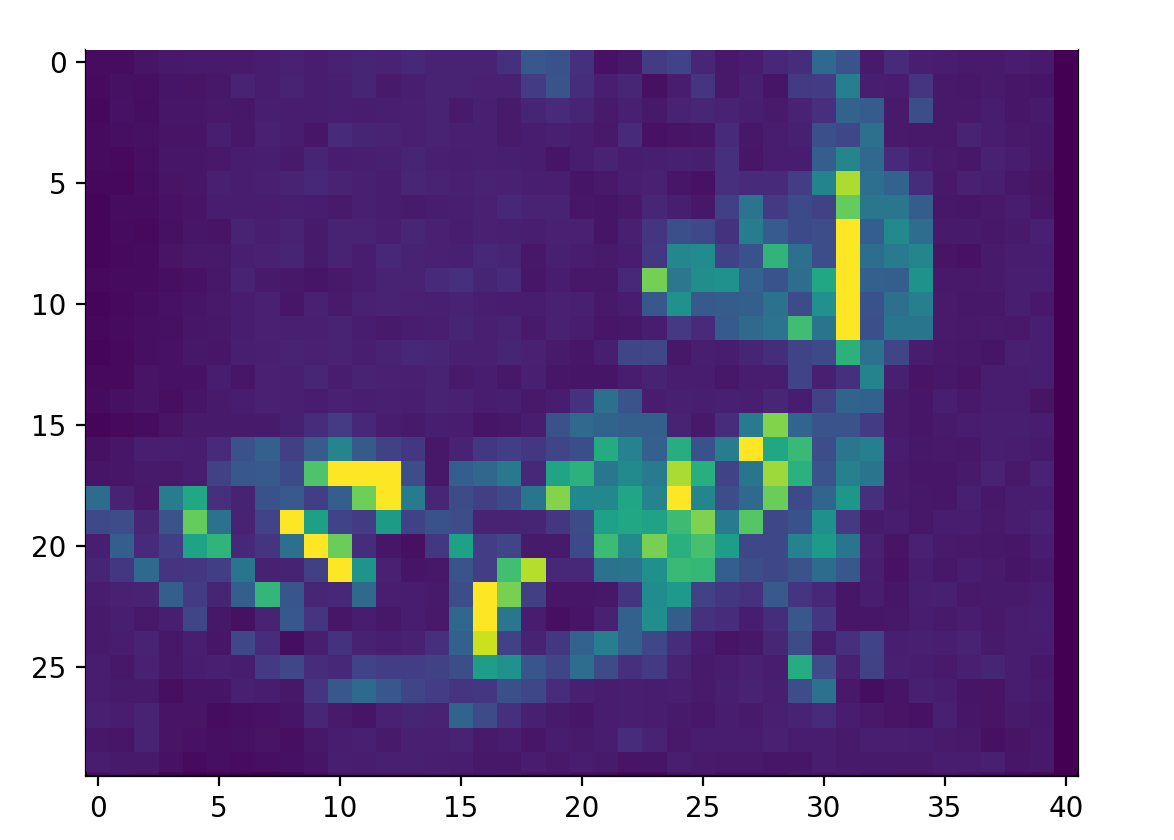
\includegraphics[scale=0.6]{Images/animation_sad.png}

{\bf Illustration 1:}  Animation of the SAD values, the lighter the color the higher the value of the SAD
\end{center}

\bigskip
 
Further the x and y vector were analyzed and also animated. But as those vectors itself are hard to use and give incomplete information, the hypotenuses were calculated with Pythagoras' theorem and displayed similar to the SAD values. The hypotenuses give information about the amount as well as the direction of the motion.
 
 \bigskip

\noindent
\begin{center}
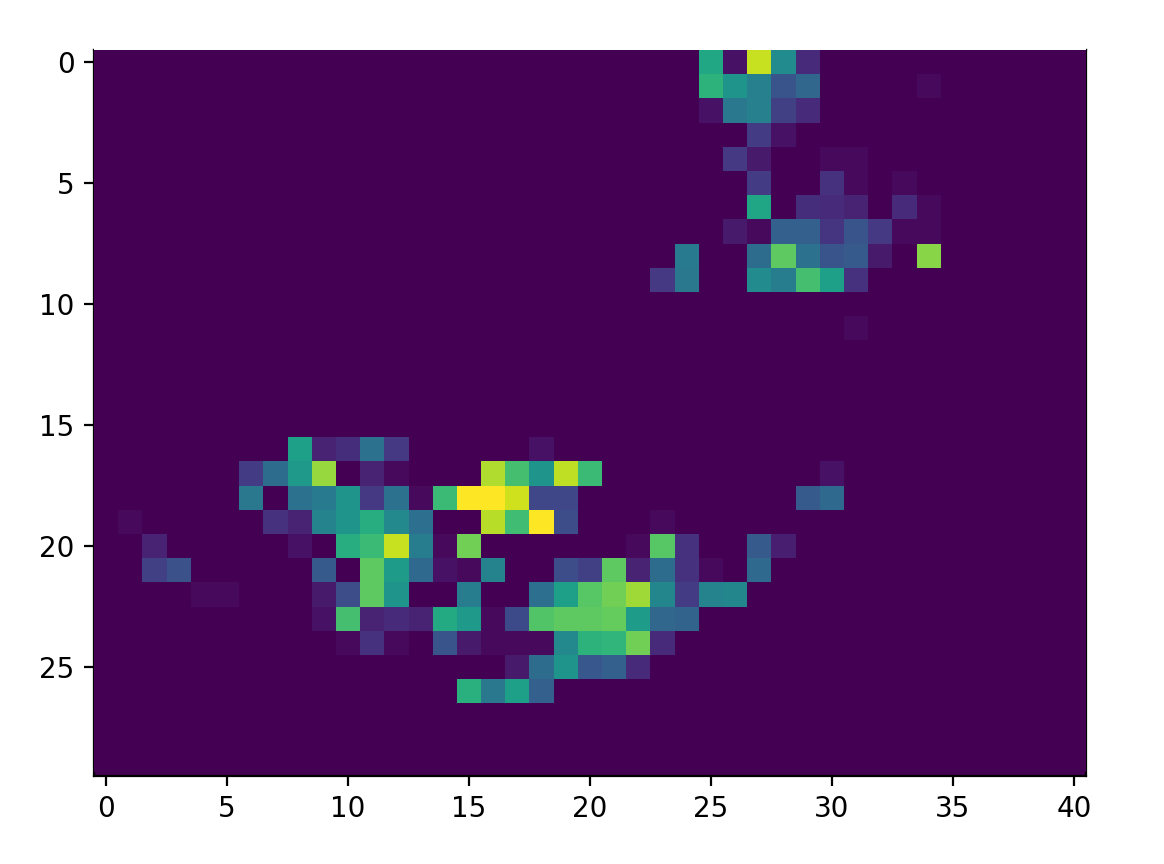
\includegraphics[scale=0.6]{Images/animation_hypotenuse.png}

{\bf Illustration 2:}  Animation of the hypotenuses, the lighter the color the higher the value of the hypotenuse
\end{center}

\bigskip

Another experimental approach was displaying the motion vectors as arrows directly in the video. This approach was helpful to get a better understanding under which conditions the best result of the motion vectors is reached.
\pagebreak

\section{Motion vectors visualized in a frame}
We used Codecvisa[4] to see how the motion vectors of a frame looks in our case.
The result is visible in Illustration 3.
\bigskip
\noindent
\begin{center}
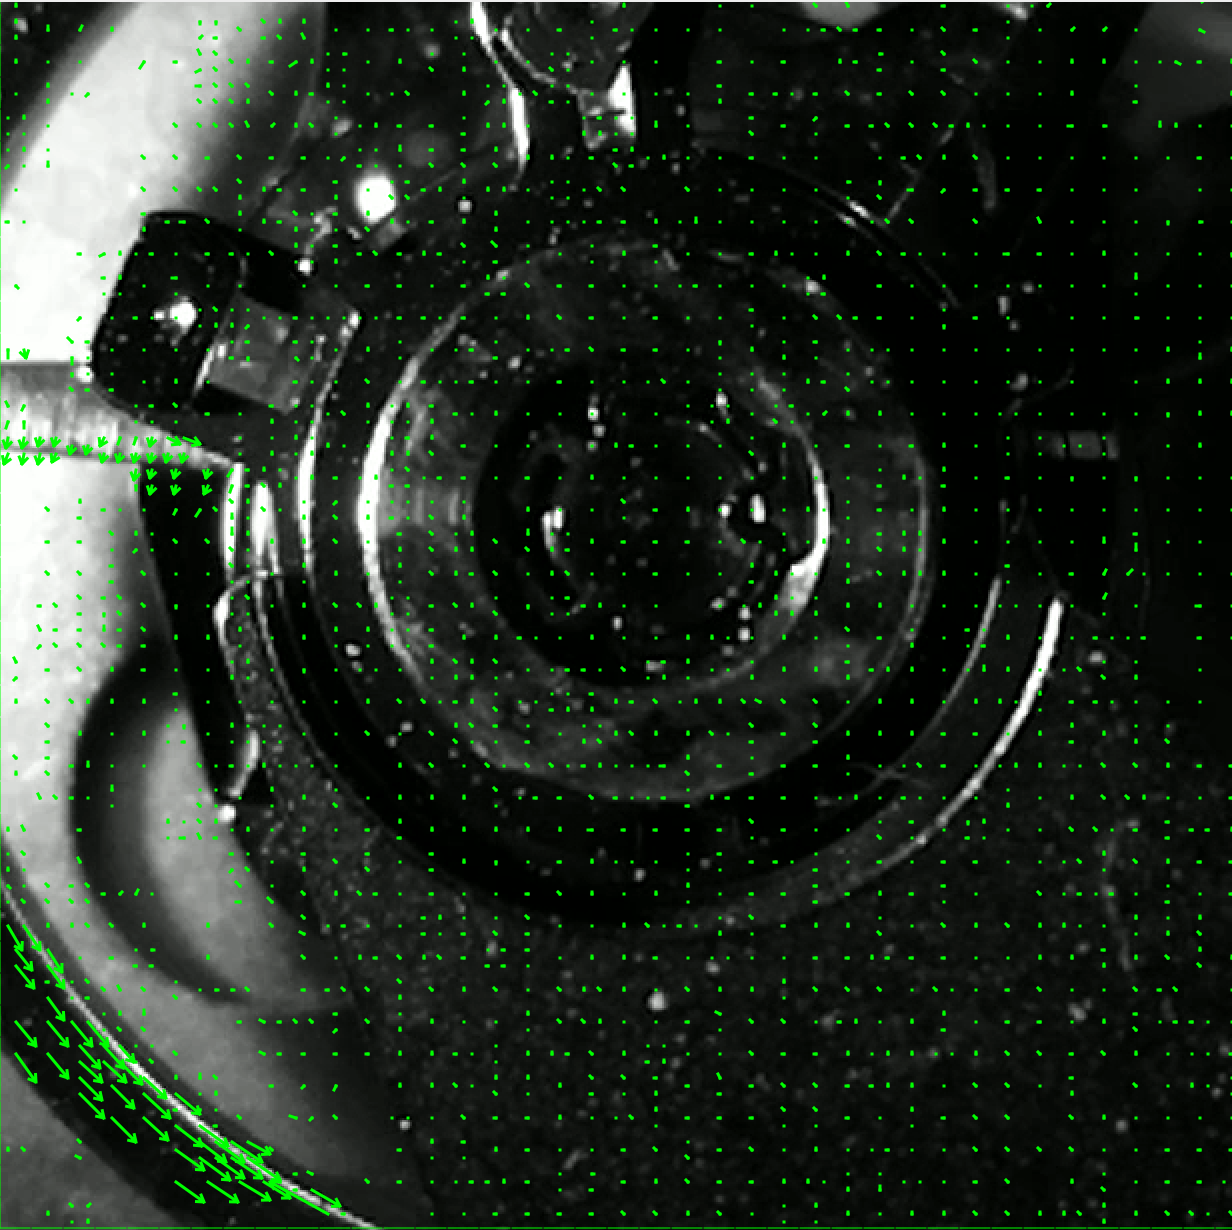
\includegraphics[scale=0.4]{Images/motion_vectors.png}

{\bf Illustration 3:}  Motion vectors drawn in one frame
\end{center}
\bigskip

We also used Excel to determine if a motion vector from one frame is the predecessor of the motion vector in the next frame.
The hope was that we could follow the moving object and thus always know the location of the object.
The result was sobering, because a frame and motion vector can not be connected to another frame and motion vector.
With this experiment, we took a look at the idea of the optical flow with the motion vectors of the mmal.

\noindent
\begin{center}
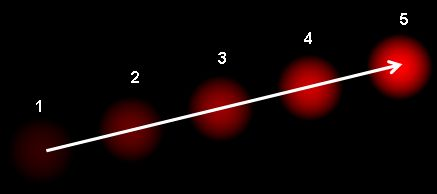
\includegraphics[scale=0.55]{Images/optical_flow_basic1.jpg}

{\bf Illustration 4:}  It shows a ball moving in 5 consecutive frames. The arrow shows its displacement vector.
\end{center}

\bigskip
\section{Crude calculation of frequency}
A crude calculation of the frequency can be made with the aid of the motion vectors and the associated time stamps per frame.
All x, y, or sad values contained in the image are summed up. If the sum of all the values is small, it is very likely that the balance wheel is not moving so it has a standstill.
For small values, the time stamp is registered and the difference to the next standstill is calculated.
Because the balance wheel makes half oscillations, it has passed from one stop to the next half a period.

Our test clock has a frequency of three Hertz. The frequency is the reciprocal of the period, which means that our period is a third.
Half of the period is equal to a standstill of the balance wheel. In this case, we should be able to measure a standstill of the balance wheel at every sixth of a second.
\pagebreak

\chapter{Appendices}


\begin{thebibliography}{9}
\bigskip
\bibitem[Uhrenwiki]{Uhrenwiki} 
(1) https://www.uhren-wiki.net/index.php?title=Zeitwaage
\bibitem[ncsli]{ncsli} https://www.ncsli.org/c/f/p11/286.314.pdf
\bibitem[chronoscop]{chronoscop} http://www.chronoskop.com/index.php/chronoskop-zeitwaagen-von-prelislisit-timegraphers/
\end{thebibliography}

\pagebreak

\section {Illustration directory}
\bigskip

\begin{itemize}
\item Abbildung 1: Animation SAD values. Linda Boedi and Valentin Bossi
\item Abbildung 2: Animation hypotenueses. Linda Boedi and Valentin Bossi
\end{itemize}

\chapter{Independence delcaration}


\end{document}
